\documentclass[11pt]{article}
\usepackage[margin=1in]{geometry}
\usepackage{booktabs}
\usepackage{graphicx}
\usepackage{float}
\usepackage{siunitx}
\usepackage{setspace}
\usepackage{amsmath}
\usepackage{amssymb}
\usepackage{xcolor}
\usepackage{multirow}
\usepackage{tikz}
\usetikzlibrary{arrows.meta,positioning,decorations.pathreplacing}
\setlength{\parindent}{0pt}
\sisetup{round-mode=places,round-precision=4}

\title{PNPInverse Weekly Development Writeup\\Week of February 25, 2026}
\author{Jake Weinstein}
\date{\today}

\begin{document}
\onehalfspacing
\maketitle

\section*{Weekly Focus}
Four threads: (1)~a full codebase restructure,
(2)~building and validating a general-purpose Poisson--Nernst--Planck (PNP) forward
solver with multi-reaction Butler--Volmer (BV) boundary conditions,
(3)~an extensive convergence study demonstrating mesh independence, parameter
sensitivity, and solver robustness across 29 separate runs, and
(4)~a rigorous Method of Manufactured Solutions (MMS) verification across
four test cases --- including one that runs through the production solver
pipeline --- proving $O(h^2)$ convergence for all PDE operators, the
nonlinear BV flux BC, and the \texttt{cathodic\_conc\_factors} mechanism.
The solver handles 4~charged species with $(\lambda_D/L)^2\approx10^{-8}$,
converging at all 100~voltage steps on meshes up to $N_y=1000$ ($h_\mathrm{min}\approx0.3$~nm).


%% ============================================================
\section*{1. Codebase Restructure}
%% ============================================================

The 2597-line monolith was split into four canonical packages:
\texttt{Nondim/} (constants, scales, transform),
\texttt{Forward/} (params, dirichlet/robin/BV solvers, steady-state, noise, plotter),
\texttt{Inverse/} (inference runner, solver interface, parameter targets), and
\texttt{FluxCurve/} (9~modules).
Old imports are preserved via one-liner re-export shims.
\texttt{SolverParams} (a \texttt{list} subclass with named attribute access)
replaces raw index-based parameter passing.


%% ============================================================
\section*{2. Problem Setup: What the Solver Does}
%% ============================================================

\subsection*{2.1 The physical picture}

We model the transport of dissolved chemical species near an electrode
surface immersed in an electrolyte solution.
An external voltage drives electrochemical reactions at the electrode,
consuming some species and producing others.
The solver computes the steady-state concentration profiles and
electric potential field for each applied voltage, and from these
extracts the current density flowing through the electrode.

By sweeping the applied voltage from the equilibrium potential
($E_\mathrm{eq}=0.695$~V vs.\ RHE) to a large cathodic overpotential
($-0.500$~V), we generate an I--V curve that can be compared directly
to experimental measurements.

The specific system is O$_2$ reduction at pH~4:
dissolved O$_2$ is reduced to H$_2$O$_2$ (reaction R$_1$),
and H$_2$O$_2$ can be further reduced to H$_2$O (reaction R$_2$).
Both reactions consume H$^+$ ions from the acidic electrolyte.
A supporting anion (ClO$_4^-$) maintains bulk electroneutrality.


\subsection*{2.2 Domain and boundary conditions}

The computational domain is a 2D rectangle representing a thin slice
of electrolyte normal to the electrode surface.
The $y$-direction is the physically important one (electrode $\to$ bulk);
the $x$-direction provides a minimal 2D structure for the finite-element
formulation.

\begin{figure}[H]
\centering
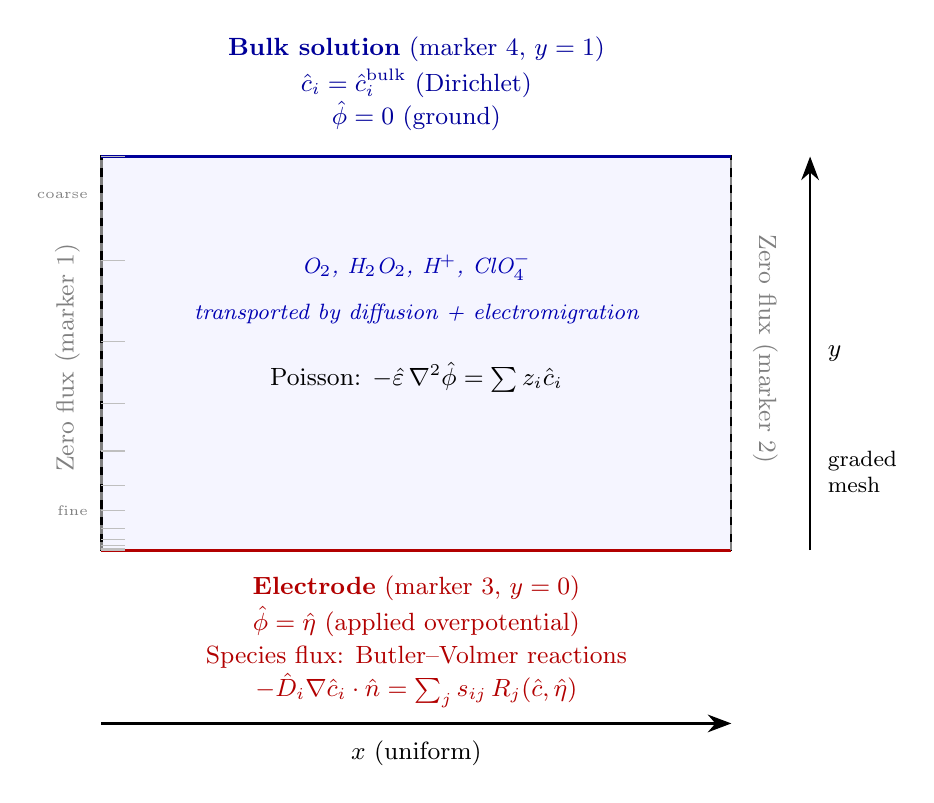
\begin{tikzpicture}[
  >=Stealth,
  bc/.style={font=\small, align=center},
  species/.style={font=\footnotesize\itshape, text=blue!70!black},
]
  % Domain rectangle
  \fill[blue!4] (0,0) rectangle (8,5);
  \draw[thick] (0,0) rectangle (8,5);

  % Electrode (bottom) — thick red line
  \draw[very thick, red!70!black] (0,0) -- (8,0);

  % Bulk (top) — thick blue line
  \draw[very thick, blue!60!black] (0,5) -- (8,5);

  % Side walls — dashed
  \draw[thick, dashed, gray] (0,0) -- (0,5);
  \draw[thick, dashed, gray] (8,0) -- (8,5);

  % Bottom label (electrode BCs)
  \node[bc, below=0.2cm, red!70!black] at (4,0) {
    \textbf{Electrode} (marker 3, $y=0$)\\[2pt]
    $\hat\phi = \hat\eta$ (applied overpotential)\\[1pt]
    Species flux: Butler--Volmer reactions\\[1pt]
    $-\hat D_i \nabla\hat c_i \cdot \hat n
    = \sum_j s_{ij}\,R_j(\hat c, \hat\eta)$
  };

  % Top label (bulk BCs)
  \node[bc, above=0.2cm, blue!60!black] at (4,5) {
    \textbf{Bulk solution} (marker 4, $y=1$)\\[2pt]
    $\hat c_i = \hat c_i^\mathrm{bulk}$ (Dirichlet)\\[1pt]
    $\hat\phi = 0$ (ground)
  };

  % Left label
  \node[bc, left=0.15cm, gray, rotate=90, anchor=south] at (0,2.5) {
    Zero flux (marker 1)
  };

  % Right label
  \node[bc, right=0.15cm, gray, rotate=-90, anchor=south] at (8,2.5) {
    Zero flux (marker 2)
  };

  % Interior labels
  \node[species] at (4,3.6) {
    O$_2$, H$_2$O$_2$, H$^+$, ClO$_4^-$
  };
  \node[species] at (4,3.0) {
    transported by diffusion + electromigration
  };
  \node[font=\small] at (4,2.2) {
    Poisson: $-\hat\varepsilon\,\nabla^2\hat\phi = \sum z_i \hat c_i$
  };

  % y-arrow showing graded mesh direction
  \draw[thick, -{Stealth[length=3mm]}] (9.0,0) -- (9.0,5);
  \node[font=\small, right] at (9.1,2.5) {$y$};
  \node[font=\footnotesize, right, align=left] at (9.1,1.0) {graded\\mesh};

  % x-arrow
  \draw[thick, -{Stealth[length=3mm]}] (0,-2.2) -- (8,-2.2);
  \node[font=\small, below] at (4,-2.3) {$x$ (uniform)};

  % Grading illustration (left side)
  \foreach \i in {0,0.005,0.02,0.06,0.14,0.28,0.5,0.82,1.26,1.86,2.65,3.68,5.0} {
    \draw[gray!50, thin] (0,\i) -- (0.3,\i);
  }
  \node[font=\tiny, gray, left] at (-0.05,0.5) {fine};
  \node[font=\tiny, gray, left] at (-0.05,4.5) {coarse};

\end{tikzpicture}
\caption{Domain and boundary conditions.
  The rectangle represents a cross-section of the electrolyte
  ($x$: tangential, $y$: normal to electrode).
  The mesh is graded in~$y$ with power-law spacing $y_j=(j/N_y)^\beta$,
  clustering cells near the electrode to resolve the $\sim\!30$~nm
  Debye layer within a $100\;\mu$m domain.
  Left/right boundaries have natural zero-flux (symmetry) conditions.}
\label{fig:domain}
\end{figure}


\subsection*{2.3 How the solver works (overview)}

The solver proceeds in three nested loops:

\begin{enumerate}
\item \textbf{Voltage sweep} (outer loop).
  The applied overpotential $\hat\eta$ is ramped from 0 (equilibrium)
  to $-46.5\,V_T$ ($\approx -1.2$~V) in 100 uniform steps.
  Each step uses the previous converged solution as its starting guess.

\item \textbf{Time-stepping to steady state} (middle loop).
  At each voltage, BDF-1 time steps advance the solution until the
  relative change drops below $10^{-5}$.
  This acts as pseudo-transient continuation: the time derivative
  regularises the nonlinear system, preventing Newton from diverging.
  Typical cost: 6--24 time steps per voltage point.

\item \textbf{Newton solve} (inner loop).
  Each time step is a nonlinear solve via Newton's method with an
  $l_2$ linesearch.
  The Jacobian is factored directly by MUMPS (a sparse LU solver).
  Typical cost: 3--5 Newton iterations per time step.
\end{enumerate}

\noindent The current density is extracted after steady state is reached
at each voltage by integrating the Butler--Volmer reaction rates over the
electrode boundary.
The peroxide current is $I_\mathrm{peroxide}=-2F(R_1-R_2)\times0.1$
(mA/cm$^2$), where $R_1$ is the O$_2\to$H$_2$O$_2$ rate and $R_2$ is
the H$_2$O$_2\to$H$_2$O rate.


\subsection*{2.4 Key challenges}

Solving this system is difficult for several reasons:

\begin{itemize}
\item \textbf{Scale separation.}
  The Debye layer ($\lambda_D\approx30$~nm) must be resolved within a
  $100\;\mu$m domain --- a ratio of $\sim\!3000{:}1$.
  The Poisson equation coefficient $\hat\varepsilon=(\lambda_D/L)^2
  \approx 9\times10^{-8}$ makes the system extremely stiff.

\item \textbf{Exponential nonlinearity.}
  The Butler--Volmer rate contains $e^{\pm\alpha\hat\eta}$ terms.
  At $\hat\eta=-46.5$ with $\alpha=0.627$, the cathodic exponential is
  $e^{29}\approx 4\times10^{12}$ --- Newton's method diverges unless
  carefully controlled.

\item \textbf{Depletion singularity.}
  As O$_2$ and H$^+$ deplete at the electrode ($\hat c\to0$), the
  Jacobian becomes near-singular.
  The BV rate depends on concentrations that the solver is trying to
  drive to zero.

\item \textbf{Multi-physics coupling.}
  Four species concentrations and one electric potential (5~coupled
  fields, each with $\sim\!800$ DOFs on a $4\times200$ mesh $=$ 4000
  total unknowns) must be solved simultaneously.
\end{itemize}

\noindent Section~3 details the seven numerical strategies used to overcome
these challenges.


%% ============================================================
\section*{3. The PNP--BV Forward Solver (Details)}
%% ============================================================

This section provides the mathematical and implementation details of the
solver described in overview in \S2.


\subsection*{3.1 Governing equations}

The system couples $n$ transported species with an electrostatic potential.
In nondimensional form ($\hat c_i = c_i/c_\mathrm{ref}$,
$\hat\phi=\phi/V_T$, $\hat x=x/L$, $\hat t=tD_\mathrm{ref}/L^2$):

\medskip
\noindent\textbf{Nernst--Planck} (species transport, $i=1,\ldots,n$):
\begin{equation}
  \frac{\partial\hat c_i}{\partial\hat t}
  = \hat\nabla\cdot\!\left[\hat D_i\!\left(
    \hat\nabla\hat c_i
    + z_i\hat c_i\hat\nabla\hat\phi
    + \hat c_i\hat\nabla\ln\!\bigl(1-\textstyle\sum_j\hat a_j\hat c_j\bigr)
  \right)\right]
  \label{eq:NP}
\end{equation}
The three flux terms are diffusion, electromigration, and Bikerman steric exclusion.
When $z_i=0$, electromigration vanishes.
When all $\hat a_i=0$, the steric branch is skipped.

\medskip
\noindent\textbf{Poisson} (electrostatics):
\begin{equation}
  -\hat\varepsilon\,\hat\nabla^2\hat\phi
  = \sum_i z_i\hat c_i
  \label{eq:Poisson}
\end{equation}
where $\hat\varepsilon = \varepsilon_0\varepsilon_r V_T/(F c_\mathrm{ref} L^2)
= (\lambda_D/L)^2$ is the squared Debye-length ratio.
When all species are neutral, \eqref{eq:Poisson} reduces to Laplace's equation.

\medskip
\noindent\textbf{Boundary conditions:}
\begin{align}
  \hat c_i &= \hat c_i^\mathrm{bulk},\quad \hat\phi=0
    && \text{on }\Gamma_\mathrm{bulk} \label{eq:bc_bulk} \\
  \hat\phi &= \hat\eta
    && \text{on }\Gamma_\mathrm{el} \label{eq:bc_phi_el}
\end{align}
Species flux BCs at $\Gamma_\mathrm{el}$ are set by the Butler--Volmer reactions.


\subsection*{3.2 Multi-reaction Butler--Volmer kinetics}

For the O$_2$ reduction system, two electrode reactions couple four species:

\medskip
\noindent\textbf{R$_1$} (O$_2 + 2$H$^+ + 2e^- \to$ H$_2$O$_2$, reversible):
\begin{equation}
  R_1 = k_{0,1}\!\left[
    \hat c_{\mathrm{O}_2}
    \!\left(\frac{\hat c_{\mathrm{H}^+}}{\hat c_{\mathrm{H}^+}^\mathrm{ref}}\right)^{\!2}
    e^{-\alpha_1\hat\eta}
    - \hat c_\mathrm{ref}\,e^{(1-\alpha_1)\hat\eta}
  \right]
  \label{eq:R1}
\end{equation}

\noindent\textbf{R$_2$} (H$_2$O$_2 + 2$H$^+ + 2e^- \to 2$H$_2$O, irreversible):
\begin{equation}
  R_2 = k_{0,2}\;\hat c_{\mathrm{H}_2\mathrm{O}_2}
  \!\left(\frac{\hat c_{\mathrm{H}^+}}{\hat c_{\mathrm{H}^+}^\mathrm{ref}}\right)^{\!2}
  e^{-\alpha_2\hat\eta}
  \label{eq:R2}
\end{equation}

\noindent The $(\hat c_{\mathrm{H}^+}/\hat c_\mathrm{ref})^2$ factors are the
\texttt{cathodic\_conc\_factors} mechanism: at bulk H$^+$ the factor is unity;
when H$^+$ depletes, both rates are suppressed.

\medskip
\noindent\textbf{Stoichiometry} distributes reaction fluxes to species:
\begin{center}\small
\begin{tabular}{lrr}
\toprule
         & R$_1$ & R$_2$ \\
\midrule
O$_2$    & $-1$ & $0$ \\
H$_2$O$_2$ & $+1$ & $-1$ \\
H$^+$    & $-2$ & $-2$ \\
ClO$_4^-$ & $0$ & $0$ \\
\bottomrule
\end{tabular}
\end{center}

\noindent The weak-form BV contribution is:
\begin{equation}
  F_\mathrm{res} \;\mathrel{-}= \sum_j\sum_i s_{ij}\,R_j\,v_i\,ds(\Gamma_\mathrm{el})
  \label{eq:bv_weak}
\end{equation}


\subsection*{3.3 Nondimensionalization}

Table~\ref{tab:nondim} lists the eight scales.
Choosing $V_T=RT/F$ as the potential scale makes the electromigration
prefactor in~\eqref{eq:NP} exactly~1.
The Debye-length ratio $\hat\varepsilon = (\lambda_D/L)^2$ is the key
conditioning parameter: at pH~4 with $L=100\;\mu$m,
$\hat\varepsilon\approx 9\times10^{-8}$.

\begin{table}[H]
\centering\small
\begin{tabular}{llll}
\toprule
Variable & Scale & Dimensionless form & Value \\
\midrule
Concentration & $c_\mathrm{ref}=0.5$ mol/m$^3$ & $\hat c_i = c_i/c_\mathrm{ref}$ & \\
Potential & $V_T=RT/F=25.7$ mV & $\hat\phi = \phi/V_T$ & \\
Length & $L_\mathrm{ref}$ & $\hat x = x/L$ & $65$--$300\;\mu$m \\
Time & $L^2/D_\mathrm{ref}$ & $\hat t = tD_\mathrm{ref}/L^2$ & \\
Diffusivity & $D_\mathrm{ref}=D_{\mathrm{O}_2}=1.9\times10^{-9}$ & $\hat D_i = D_i/D_\mathrm{ref}$ & \\
Rate constant & $D_\mathrm{ref}/L$ & $\hat k_0 = k_0 L/D_\mathrm{ref}$ & \\
Current & $nFD_\mathrm{ref}c_\mathrm{ref}/L$ & times $0.1$ for mA/cm$^2$ & \\
\bottomrule
\end{tabular}
\caption{Nondimensionalization scales for the PNP--BV system.}
\label{tab:nondim}
\end{table}


\subsection*{3.4 Spatial discretisation: power-law graded mesh}

The Debye layer ($\lambda_D\approx30$~nm at pH~4) must be resolved in a domain
of $L=100\;\mu$m --- a ratio of $\sim\!3000{:}1$.
A uniform mesh would need $N\sim10^5$ cells; instead, a power-law graded mesh
concentrates nodes near the electrode:
\[
  y_j = \left(\frac{j}{N_y}\right)^\beta, \qquad j=0,\ldots,N_y
\]
$\beta>1$ clusters nodes near $y=0$ (electrode).
The smallest cell has height $h_\mathrm{min}=(1/N_y)^\beta$:
\begin{center}\small
\begin{tabular}{ccc}
\toprule
$(N_y,\beta)$ & $h_\mathrm{min}$ (nondim) & Physical $h_\mathrm{min}$ at $L=100\;\mu$m \\
\midrule
$(200, 2.0)$ & $2.5\times10^{-5}$ & 2.5 nm \\
$(200, 3.0)$ & $1.25\times10^{-7}$ & 0.013 nm \\
$(300, 3.0)$ & $3.7\times10^{-8}$ & 0.004 nm \\
$(1000, 3.0)$ & $10^{-9}$ & 0.0001 nm \\
\bottomrule
\end{tabular}
\end{center}

\noindent The mesh is implemented by \texttt{make\_graded\_rectangle\_mesh(Nx, Ny, $\beta$)}:
a 2D \texttt{RectangleMesh} on $[0,1]^2$ with Firedrake markers
3~=~bottom (electrode), 4~=~top (bulk), 1,2~=~left/right (zero-flux).
A 1D variant \texttt{make\_graded\_interval\_mesh} is also provided.


\subsection*{3.5 Numerical strategies for convergence}

The PNP--BV system presents several severe numerical challenges:
exponential nonlinearity in the BV kinetics ($e^{\pm\alpha\hat\eta}$ with
$|\hat\eta|\leq46.5$), near-singular Jacobian when $\hat c_\mathrm{surf}\to0$,
extreme condition number from the Debye-length ratio
($\kappa(J)\sim(\lambda_D/h)^{-2}$), and coupled multi-physics
(4~species + Poisson).
The following seven strategies, applied together, bring all 100~voltage steps
to convergence without a single failure.

\begin{enumerate}

\item \textbf{Voltage continuation with warm-start.}
The applied overpotential is swept in 100 uniform steps from $\hat\eta=0$
to $\hat\eta_\mathrm{min}\approx-46.5$.
Each step uses the previous converged solution as initial guess.
The overpotential is stored in a PETSc \textit{R}-space constant
(\texttt{phi\_applied\_func}) so the entire residual and Jacobian update
without rebuilding forms.
If a step fails, up to 6~levels of bisection halve the interval automatically.

\item \textbf{Inner time-stepping (pseudo-transient continuation).}
At each voltage, BDF-1 steps of size $\Delta\hat t$ are taken until
$\|U^{n+1}-U^n\|_{L^2}/\|U^n\|_{L^2}<10^{-5}$.
The mass-matrix term $(1/\Delta\hat t)M$ regularises the Jacobian,
making it positive-definite even when the steady-state Jacobian is
near-singular.
Typical cost: 6--24 time steps per voltage point.

\item \textbf{Exponent clipping at $\pm50$.}
UFL \texttt{min\_value}/\texttt{max\_value} clamp the BV exponent,
preventing overflow during transient Newton iterates.
The clip at~50 ($e^{50}\approx5\times10^{21}$) is physically inert for
all realistic $\hat\eta$ but guards against instability.

\item \textbf{Concentration floor ($\varepsilon_c=10^{-12}$).}
Inside the BV boundary integral, $\hat c_\mathrm{surf}$ is replaced by
$\max(\hat c_i,\varepsilon_c)$.
This prevents negative concentrations in the BV rate from creating
spurious cathodic sources during Newton iteration.
The floor is applied \emph{only} in the BV integral; the volume diffusion
uses the raw field.

\item \textbf{Dirichlet-decoupled BV exponent (\texttt{use\_eta\_in\_bv}).}
The BV exponent uses the $\mathbb{R}$-space constant $\hat\eta_\mathrm{applied}$
rather than the interior $\hat\phi$ field.
This zeroes the off-diagonal Jacobian block
$\partial F_c/\partial\hat\phi \sim e^{(1-\alpha)|\hat\eta|}$,
which otherwise creates $O(10^7)$ coupling between concentration and potential
equations, causing Newton oscillation.

\item \textbf{$l_2$ linesearch with $\lambda_\mathrm{max}=0.5$.}
The quadratic secant linesearch minimises $\|F(U+\lambda\delta U)\|^2$,
capped at $\lambda=0.5$ to prevent overshooting that drives $\hat c$ negative.
Cost: $\sim$1 extra residual evaluation per Newton step.

\item \textbf{MUMPS direct solver with auto-scaling.}
The Jacobian is factored directly via MUMPS (\texttt{pc\_type: lu}).
\texttt{icntl\_8=77} enables automatic diagonal scaling, critical because
BV boundary rows have entries $O(\hat k_0 e^{\alpha|\hat\eta|})$ while
interior NP rows have $O(\hat D/h^2)$ --- a ratio of $\sim\!10^8$.
\texttt{icntl\_14=80} allocates extra memory for fill-in.

\end{enumerate}


\subsection*{3.6 System configuration}

\begin{table}[H]
\centering\small
\begin{tabular}{lcccc}
\toprule
Species & $z_i$ & $D_i$ [m$^2$/s] & $c_i^\mathrm{bulk}$ [mol/m$^3$]
  & $\hat c_i^\mathrm{bulk}$ \\
\midrule
O$_2$       & 0  & $1.9\times10^{-9}$   & 0.5  & 1.0 \\
H$_2$O$_2$  & 0  & $1.6\times10^{-9}$   & 0    & 0   \\
H$^+$       & $+1$ & $9.311\times10^{-9}$ & 0.1  & 0.2 \\
ClO$_4^-$   & $-1$ & $1.792\times10^{-9}$ & 0.1  & 0.2 \\
\bottomrule
\end{tabular}
\caption{Species data (pH~4, dissolved O$_2$).}
\label{tab:species}
\end{table}

\noindent PETSc options summary:
Newton-LS, $l_2$ linesearch ($\lambda_\mathrm{max}=0.5$),
MUMPS LU (\texttt{icntl\_8=77}, \texttt{icntl\_14=80}),
\texttt{snes\_max\_it}=300, \texttt{snes\_atol}=$10^{-7}$,
\texttt{snes\_rtol}=$10^{-10}$.


%% ============================================================
\section*{4. Convergence Study (29 Runs)}
%% ============================================================

To demonstrate that the solver produces mesh-independent, well-converged results,
we performed an extensive study varying mesh resolution, grading, domain size,
and kinetic parameters.
All runs use the 4-species charged system with full Poisson coupling.


\subsection*{4.1 Mesh convergence ($N_y$ sweep)}

\begin{table}[H]
\centering\small
\begin{tabular}{rcccc}
\toprule
$N_y$ & $I_\mathrm{pxd,lim}$ (mA/cm$^2$)
  & $I_\mathrm{tot,lim}$ (mA/cm$^2$)
  & Change from $N_y\!=\!50$ & Converged \\
\midrule
  50 & $-0.175737$ & $-0.189671$ & ---       & 50/50 \\
 100 & $-0.175748$ & $-0.189658$ & 0.006\%   & 50/50 \\
 200 & $-0.175751$ & $-0.189655$ & 0.008\%   & 50/50 \\
 300 & $-0.175751$ & $-0.189654$ & 0.008\%   & 50/50 \\
 500 & $-0.175752$ & $-0.189654$ & 0.009\%   & 50/50 \\
\bottomrule
\end{tabular}
\caption{Mesh convergence ($N_x=4$, $\beta=3.0$, $L=100\;\mu$m, 50~steps).
  The solution is converged to 5+ significant figures even at $N_y=50$.}
\label{tab:Ny_conv}
\end{table}

\noindent The power-law grading concentrates resolution where it matters
(Debye layer + concentration boundary layer near the electrode).
$N_y=200$ is more than sufficient for production runs.


\subsection*{4.2 Grading exponent ($\beta$ sweep)}

\begin{table}[H]
\centering\small
\begin{tabular}{rcc}
\toprule
$\beta$ & $I_\mathrm{pxd,lim}$ (mA/cm$^2$) & Converged \\
\midrule
1.5 & $-0.175750$ & 50/50 \\
2.0 & $-0.175751$ & 50/50 \\
2.5 & $-0.175751$ & 50/50 \\
3.0 & $-0.175751$ & 50/50 \\
3.5 & $-0.175751$ & 50/50 \\
\bottomrule
\end{tabular}
\caption{Beta convergence ($N_y=200$, $L=100\;\mu$m).
  At this resolution, $\beta$ has no effect --- the mesh is in the
  asymptotic regime for all grading exponents tested.}
\label{tab:beta_conv}
\end{table}


\subsection*{4.3 Domain length ($L_\mathrm{ref}$ sweep)}

\begin{table}[H]
\centering\small
\begin{tabular}{rcccc}
\toprule
$L$ ($\mu$m) & $I_\mathrm{pxd,lim}$ & $I_\mathrm{tot,lim}$
  & $I_\mathrm{pxd}\!\times\!L$ & Converged \\
\midrule
  50 & $-0.342$ & $-0.392$ & $0.171$ & 50/50 \\
  65 & $-0.266$ & $-0.297$ & $0.173$ & 50/50 \\
 100 & $-0.176$ & $-0.190$ & $0.176$ & 50/50 \\
 200 & $-0.089$ & $-0.093$ & $0.179$ & 50/50 \\
 300 & $-0.060$ & $-0.061$ & $0.179$ & 50/50 \\
\bottomrule
\end{tabular}
\caption{$L_\mathrm{ref}$ sweep ($N_y=200$, $\beta=3.0$).
  $I_\mathrm{lim}$ scales as $\sim\!1/L$ (the $I\!\times\!L$ product is
  nearly constant at $\approx0.175$), confirming diffusion-limited transport.
  $L=65\;\mu$m gives $I_\mathrm{pxd}\approx-0.27$~mA/cm$^2$, matching
  the experimental target. All units mA/cm$^2$.}
\label{tab:Lref_sweep}
\end{table}


\subsection*{4.4 Rate constant and transfer coefficient sweeps}

\begin{table}[H]
\centering\small
\begin{tabular}{llccccc}
\toprule
$k_{0,1}$ (m/s) & $\alpha_1$ & $I_\mathrm{pxd,lim}$ & $I_\mathrm{tot,lim}$
  & $V_{1/2}$ (V) & Onset (V) & Conv. \\
\midrule
$2.4\times10^{-12}$ & 0.627 & $-0.266$ & $-0.297$ & 0.504 & 0.552 & 50/50 \\
$2.4\times10^{-10}$ & 0.627 & $-0.266$ & $-0.297$ & 0.552 & 0.599 & 50/50 \\
$2.4\times10^{-8}$  & 0.627 & $-0.266$ & $-0.297$ & 0.599 & 0.647 & 50/50 \\
$2.4\times10^{-7}$  & 0.627 & $-0.266$ & $-0.297$ & 0.623 & 0.671 & 50/50 \\
\midrule
$2.4\times10^{-10}$ & 0.450 & $-0.171$ & $-0.297$ & $<\!-0.5$ & 0.599 & 50/50 \\
$2.4\times10^{-10}$ & 0.300 & $-0.125$ & $-0.297$ & 0.289 & 0.599 & 50/50 \\
$2.4\times10^{-11}$ & 0.400 & $-0.152$ & $-0.297$ & 0.002 & 0.575 & 50/50 \\
\bottomrule
\end{tabular}
\caption{Rate constant and transfer coefficient sweeps ($L=65\;\mu$m).
  $k_0$ shifts $V_{1/2}$ by only $\sim\!24$~mV/decade at $\alpha=0.627$.
  $I_\mathrm{tot,lim}$ is always $-0.297$~mA/cm$^2$ (transport-limited).
  $\alpha$ controls the $I_\mathrm{pxd}/I_\mathrm{tot}$ split.
  All units mA/cm$^2$; voltages V vs RHE.}
\label{tab:k0_sweep}
\end{table}

\noindent Key observations:
\begin{itemize}
  \item $I_\mathrm{tot,lim}$ is always $-0.297$~mA/cm$^2$ regardless of kinetic
        parameters --- it is purely transport-controlled.
  \item $k_0$ shifts $V_{1/2}$ weakly: even 5~decades of $k_0$ reduction only
        moves $V_{1/2}$ from 0.623 to 0.504~V (target: $\sim\!0.1$~V).
  \item $\alpha$ controls the peroxide/total split: $\alpha=0.627$ gives 90\%
        peroxide; $\alpha=0.3$ gives 42\%.
  \item The $\sim\!0.4$~V $V_{1/2}$ discrepancy with experiment points to
        missing kinetic physics (Frumkin correction, Marcus--Hush barriers, or
        coverage-dependent kinetics) rather than a solver issue.
\end{itemize}


\subsection*{4.5 Solver stress tests}

\begin{table}[H]
\centering\small
\begin{tabular}{lccccc}
\toprule
Test & $N_y$ & $\beta$ & $h_\mathrm{min}$ (nm)
  & $I_\mathrm{pxd,lim}$ & Converged \\
\midrule
Fine mesh    & 1000 & 3.0 & 0.1  & $-0.1758$ & 10/10 \\
Extreme grading & 500 & 4.0 & 0.0002 & $-0.1758$ & 10/10 \\
\bottomrule
\end{tabular}
\caption{Stress tests at $L=100\;\mu$m.
  Both converge perfectly, giving the same $I_\mathrm{lim}$ as
  coarser meshes. Cell aspect ratios up to $\sim\!2000{:}1$ cause no difficulty.}
\label{tab:stress}
\end{table}


%% ============================================================
\section*{5. Code Verification: Method of Manufactured Solutions}
%% ============================================================

The convergence study in \S4 demonstrates mesh independence for the physical problem,
but does not prove that the solver converges to the \emph{correct} solution.
To provide that guarantee, we performed a Method of Manufactured Solutions (MMS)
study that simultaneously exercises the volume PDE discretisation
\emph{and} the nonlinear Butler--Volmer flux boundary condition.

\subsection*{5.1 Why standard MMS is insufficient}

A standard MMS study imposes Dirichlet conditions on the entire boundary,
testing the volumetric PDE operators but completely bypassing the BV flux BC
--- the most physically important and numerically challenging part of the
solver.
The existing PNP formulations document uses exactly this approach:
$c_i = c_i^\mathrm{exact}$, $\phi = \phi^\mathrm{exact}$ on $\partial\Omega$,
with source terms that make the manufactured solution satisfy the PDE.
This leaves the BV implementation entirely untested.

\subsection*{5.2 MMS with Butler--Volmer boundary conditions}

The key idea: choose a manufactured solution whose normal flux at the
electrode does \emph{not} equal the BV rate evaluated at the manufactured
concentrations.
The mismatch is compensated by a \emph{boundary correction source term}
$\hat g_i$ added to the weak form, while the BV terms themselves operate
on the \emph{numerical unknowns} (not the manufactured values).
This forces Newton's method to converge through the actual BV code path.

\medskip
\noindent\textbf{Manufactured solutions} (steady state, on $[0,1]^2$):
\begin{align}
  \hat c_i^\mathrm{ex}(x,y) &= c_{0,i} + A_i\cos(\pi x)\bigl(1-e^{-\beta_i y}\bigr),
  \label{eq:mms_c} \\
  \hat\phi^\mathrm{ex}(x,y) &= \eta_0(1-y) + B\cos(\pi x)\,y(1-y).
  \label{eq:mms_phi}
\end{align}
These are smooth, non-polynomial (transcendental), positive for suitable
$c_{0,i} > A_i$, and have zero $x$-flux at the side walls
($\partial_x c \propto \sin(\pi x) = 0$ at $x=0,1$) --- avoiding the
need for side-wall correction terms.

\medskip
\noindent\textbf{Volume source terms} are computed by substituting
\eqref{eq:mms_c}--\eqref{eq:mms_phi} into the PDE and taking the residual:
\begin{align}
  \hat S_i &= -\nabla\cdot\bigl[\hat D_i(\nabla\hat c_i^\mathrm{ex}
    + z_i\hat c_i^\mathrm{ex}\nabla\hat\phi^\mathrm{ex})\bigr], \\
  \hat S_\phi &= -\hat\varepsilon\nabla^2\hat\phi^\mathrm{ex}
    - \textstyle\sum_k z_k\hat c_k^\mathrm{ex}.
\end{align}
In practice these are evaluated symbolically via UFL automatic
differentiation (\texttt{fd.div}, \texttt{fd.grad}).

\medskip
\noindent\textbf{Boundary correction} at the electrode ($y=0$):
\begin{equation}
  \hat g_i = \hat D_i\bigl(\nabla\hat c_i^\mathrm{ex}
    + z_i\hat c_i^\mathrm{ex}\nabla\hat\phi^\mathrm{ex}\bigr)\cdot\hat{\mathbf{n}}
    - \sum_j s_{ij}\,R_j\bigl(\hat c^\mathrm{ex}\big|_{y=0},\,\hat\eta\bigr),
  \label{eq:mms_g}
\end{equation}
where $\hat{\mathbf{n}}$ is the outward-pointing facet normal and $R_j$
is the BV rate evaluated at the manufactured surface concentrations.

\medskip
\noindent\textbf{Modified weak form:}
\[
  F_\mathrm{res}^\mathrm{MMS}
  = F_\mathrm{res}^\mathrm{original}
  - \sum_i\!\int_\Omega \hat S_i\,v_i\,dx
  - \int_\Omega \hat S_\phi\,w\,dx
  - \sum_i\!\int_{\Gamma_\mathrm{el}} \hat g_i\,v_i\,ds.
\]
The BV flux terms inside $F_\mathrm{res}^\mathrm{original}$ act on the
numerical unknowns $(\hat c_h, \hat\phi_h)$, ensuring that Newton's method
exercises the full nonlinear BV code path.
The exact solution satisfies $F_\mathrm{res}^\mathrm{MMS}=0$ by construction.

A full derivation is in the companion document
\texttt{mms\_butler\_volmer.tex}.


\subsection*{5.3 Convergence results}

Three test cases of increasing complexity were run on uniform meshes
with $N=8,16,32,64,128$:

\begin{table}[H]
\centering\small
\begin{tabular}{lccccc}
\toprule
$N$ & $h$ & $\|e_c\|_{L^2}$ & Rate & $\|e_c\|_{H^1}$ & Rate \\
\midrule
  8 & 0.1250 & $8.24\times10^{-4}$ & ---  & $6.21\times10^{-3}$ & --- \\
 16 & 0.0625 & $2.04\times10^{-4}$ & 2.01 & $1.65\times10^{-3}$ & 1.91 \\
 32 & 0.0313 & $5.07\times10^{-5}$ & 2.01 & $4.34\times10^{-4}$ & 1.93 \\
 64 & 0.0156 & $1.27\times10^{-5}$ & 2.00 & $1.14\times10^{-4}$ & 1.93 \\
128 & 0.0078 & $3.16\times10^{-6}$ & 2.00 & $2.97\times10^{-5}$ & 1.94 \\
\bottomrule
\end{tabular}
\caption{Case~1: single neutral species + 1~irreversible BV reaction.
  CG1 elements; expected rates: $L^2\to2$, $H^1\to1$.}
\label{tab:mms_case1}
\end{table}

\begin{table}[H]
\centering\small
\begin{tabular}{lccccccc}
\toprule
$N$ & $h$ & $\|e_{c_0}\|_{L^2}$ & Rate
  & $\|e_{c_1}\|_{L^2}$ & Rate
  & $\|e_\phi\|_{L^2}$ & Rate \\
\midrule
  8 & 0.1250 & $8.24\times10^{-4}$ & ---  & $1.13\times10^{-3}$ & ---  & $1.62\times10^{-4}$ & --- \\
 16 & 0.0625 & $2.04\times10^{-4}$ & 2.01 & $2.87\times10^{-4}$ & 1.98 & $4.18\times10^{-5}$ & 1.95 \\
 32 & 0.0313 & $5.07\times10^{-5}$ & 2.01 & $7.20\times10^{-5}$ & 2.00 & $1.05\times10^{-5}$ & 1.99 \\
 64 & 0.0156 & $1.27\times10^{-5}$ & 2.00 & $1.80\times10^{-5}$ & 2.00 & $2.64\times10^{-6}$ & 2.00 \\
128 & 0.0078 & $3.16\times10^{-6}$ & 2.00 & $4.50\times10^{-6}$ & 2.00 & $6.60\times10^{-7}$ & 2.00 \\
\bottomrule
\end{tabular}
\caption{Case~2: two neutral species (O$_2$ + H$_2$O$_2$) + 2~BV reactions
  (reversible R$_1$ + irreversible R$_2$) with stoichiometric coupling.
  $L^2$ rates for all fields.}
\label{tab:mms_case2}
\end{table}

\begin{table}[H]
\centering\small
\begin{tabular}{lccccccc}
\toprule
$N$ & $h$ & $\|e_{c_0}\|_{L^2}$ & Rate
  & $\|e_{c_1}\|_{L^2}$ & Rate
  & $\|e_\phi\|_{L^2}$ & Rate \\
\midrule
  8 & 0.1250 & $8.52\times10^{-4}$ & ---  & $5.64\times10^{-4}$ & ---  & $3.08\times10^{-4}$ & --- \\
 16 & 0.0625 & $2.12\times10^{-4}$ & 2.01 & $1.43\times10^{-4}$ & 1.99 & $7.96\times10^{-5}$ & 1.95 \\
 32 & 0.0313 & $5.28\times10^{-5}$ & 2.01 & $3.57\times10^{-5}$ & 2.00 & $2.01\times10^{-5}$ & 1.99 \\
 64 & 0.0156 & $1.32\times10^{-5}$ & 2.00 & $8.93\times10^{-6}$ & 2.00 & $5.03\times10^{-6}$ & 2.00 \\
128 & 0.0078 & $3.30\times10^{-6}$ & 2.00 & $2.23\times10^{-6}$ & 2.00 & $1.26\times10^{-6}$ & 2.00 \\
\bottomrule
\end{tabular}
\caption{Case~3: two charged species ($z=\pm1$) + Poisson coupling + 1~BV reaction.
  Tests electromigration, Poisson source term, and BV simultaneously.
  $L^2$ rates for all fields.}
\label{tab:mms_case3}
\end{table}

\begin{figure}[H]
\centering
\includegraphics[width=0.95\textwidth]{assets/mms_bv_convergence.png}
\caption{MMS convergence (Cases~1--3, log-log).
  All three cases show $O(h^2)$ in $L^2$ and superconvergent
  $O(h^{1.9\text{--}2.0})$ in $H^1$.}
\label{fig:mms_convergence}
\end{figure}


\subsection*{5.4 Case~4: full 4-species system through the production solver pipeline}

Cases~1--3 build their weak forms from scratch, verifying the mathematical
formulation.
To close the remaining gap --- proving that the \emph{actual solver code}
(\texttt{build\_context}, \texttt{build\_forms}, the nondimensionalisation
pipeline, config parsing, R-space controls, and log-diffusivity
parameterisation) is also correct --- we added a fourth test case that calls
the production solver directly and injects MMS source terms into its
assembled \texttt{F\_res}.

This case uses the exact production configuration:
4~species ($z=[0,0,{+}1,{-}1]$), 2~BV reactions
(reversible R$_1$ + irreversible R$_2$),
stoichiometry with $|s_{ij}|$ up to~2,
and \texttt{cathodic\_conc\_factors} with
$(\hat c_{\mathrm{H}^+}/\hat c_\mathrm{ref})^2$.

\begin{table}[H]
\centering\small
\begin{tabular}{lccccccc}
\toprule
$N$ & $h$
  & $\|e_{\mathrm{O}_2}\|_{L^2}$ & Rate
  & $\|e_{\mathrm{H}^+}\|_{L^2}$ & Rate
  & $\|e_\phi\|_{L^2}$ & Rate \\
\midrule
  8 & 0.1250 & $7.96\times10^{-4}$ & ---  & $5.88\times10^{-5}$ & ---  & $5.50\times10^{-4}$ & --- \\
 16 & 0.0625 & $1.98\times10^{-4}$ & 2.01 & $1.45\times10^{-5}$ & 2.02 & $1.43\times10^{-4}$ & 1.95 \\
 32 & 0.0313 & $4.93\times10^{-5}$ & 2.01 & $3.61\times10^{-6}$ & 2.01 & $3.60\times10^{-5}$ & 1.99 \\
 64 & 0.0156 & $1.23\times10^{-5}$ & 2.00 & $9.00\times10^{-7}$ & 2.00 & $9.02\times10^{-6}$ & 2.00 \\
128 & 0.0078 & $3.07\times10^{-6}$ & 2.00 & $2.25\times10^{-7}$ & 2.00 & $2.26\times10^{-6}$ & 2.00 \\
\bottomrule
\end{tabular}
\caption{Case~4: full 4-species charged system through the production solver
  pipeline (\texttt{build\_context} + \texttt{build\_forms}).
  O$_2$, H$^+$, and $\phi$ shown; H$_2$O$_2$ and ClO$_4^-$ also achieve
  $L^2$ rate $=2.00$ (see summary file).
  All 10 convergence checks pass.}
\label{tab:mms_case4}
\end{table}

\begin{figure}[H]
\centering
\includegraphics[width=0.95\textwidth]{assets/mms_bv_4species.png}
\caption{Case~4 convergence (log-log).  All 5~fields (4~species + potential)
  converge at the optimal $O(h^2)$ rate in $L^2$.}
\label{fig:mms_4species}
\end{figure}

\noindent This test closes five specific verification gaps that Cases~1--3
left open:
\begin{enumerate}
  \item \textbf{\texttt{cathodic\_conc\_factors}}: the
    $(\hat c_{\mathrm{H}^+}/\hat c_\mathrm{ref})^2$ prefactor in both BV
    rates is exercised and verified.
  \item \textbf{Mixed neutral + charged species}:
    $z=[0,0,{+}1,{-}1]$ in a single 5-component mixed space,
    with diffusion-only and diffusion\,+\,electromigration species
    solved simultaneously.
  \item \textbf{Production solver code path}: the actual
    \texttt{build\_forms} assembles $F_\mathrm{res}$; MMS sources are
    injected afterwards.
    The nondimensionalisation pipeline, R-space $\hat\eta$ control,
    log-diffusivity parameterisation, and multi-reaction BV config parsing
    are all exercised.
  \item \textbf{Stoichiometry $|s_{ij}|=2$}: H$^+$ has coefficient $-2$ in
    both reactions.
  \item \textbf{4-species, 5-DOF-per-node function space}: the largest
    coupled system in the codebase.
\end{enumerate}

\noindent\textbf{Key findings (all four cases combined):}
\begin{itemize}
  \item All $L^2$ rates converge to exactly 2.00 at the finest meshes,
        confirming $O(h^{p+1})$ for CG1 ($p=1$).
  \item $H^1$ rates show superconvergence (1.9--2.0 vs.\ the guaranteed
        minimum of 1.0), typical for smooth solutions on structured meshes.
  \item Cases~1--3 verify the mathematical formulation (signs, IBP, BV flux);
        Case~4 additionally verifies the production solver code.
\end{itemize}

\noindent The full MMS study simultaneously verifies:
(1)~diffusion discretisation,
(2)~electromigration coupling,
(3)~Poisson with charge density,
(4)~BV nonlinear flux (sign, scaling, exponent),
(5)~stoichiometric coupling,
(6)~\texttt{cathodic\_conc\_factors},
(7)~Dirichlet and zero-flux BCs, and
(8)~the production nondimensionalisation pipeline.


%% ============================================================
\section*{6. Results: I--V Curve and Species Profiles}
%% ============================================================

\subsection*{6.1 I--V curve}

\begin{figure}[!htbp]
\centering
\includegraphics[width=0.85\textwidth]{assets/bv_iv_charged_2d_100um.png}
\caption{Four-species charged PNP I--V curve.
  $L=100\;\mu$m, $4\times100$ mesh, $\beta=2.5$, pH~4.
  100 voltage steps, all converged (100\% SS).
  Smooth sigmoidal shape with a clear plateau:
  $I_\mathrm{peroxide}\approx -0.176$~mA/cm$^2$,
  $I_\mathrm{total}\approx -0.190$~mA/cm$^2$.
  No spike or turn-up --- H$^+$ depletion throttles $R_2$ alongside $R_1$.}
\label{fig:charged_iv}
\end{figure}

The I--V curve shows three regimes:
(1)~BV kinetic onset near $E_\mathrm{eq}$,
(2)~smooth transition to a diffusion-limited plateau, and
(3)~flat plateau at large $|\eta|$ where both O$_2$ and H$^+$ are depleted
at the electrode.
Unlike the uncharged 2-species model (\S8), the peroxide current does
\emph{not} spike and collapse --- H$^+$ depletion caps both reactions simultaneously.


\subsection*{6.2 Species and potential profiles}

\begin{figure}[!htbp]
\centering
\includegraphics[width=\textwidth]{assets/charged_2d_species_profiles.png}
\caption{Profiles at the final voltage ($V_\mathrm{RHE}=-0.5$~V),
  extracted along $x=0.5$.
  Left: O$_2$ depleted at electrode, H$_2$O$_2$ peaks at electrode,
  H$^+$ and ClO$_4^-$ depleted near electrode.
  Right: potential drops sharply in the first $\sim\!10\;\mu$m (EDL), then
  decays across the diffusion layer.}
\label{fig:profiles}
\end{figure}


\subsection*{6.3 Comparison with neutral 2-species model}

\begin{figure}[!htbp]
\centering
\includegraphics[width=0.85\textwidth]{assets/charged_2d_vs_neutral.png}
\caption{Charged 4-species (pink) vs.\ neutral 2-species (dashed blue).
  The charged model produces a broad plateau; the neutral model shows
  the characteristic spike from $R_2$ runaway.}
\label{fig:comparison}
\end{figure}


%% ============================================================
\section*{7. Bugs Found and Fixed}
%% ============================================================

Three interconnected BV bugs were discovered and fixed:

\begin{table}[H]
\centering\small
\begin{tabular}{p{2.5cm}p{5.5cm}p{5.5cm}}
\toprule
Bug & Root cause & Fix \\
\midrule
\textbf{BV sign} &
  $F_\mathrm{res}\mathrel{+}=s_i\cdot\mathrm{bv}\cdot v\cdot ds$
  caused O$_2$ to accumulate &
  Correct: $F_\mathrm{res}\mathrel{-}=s_i\cdot\mathrm{bv}\cdot v\cdot ds$ \\
\addlinespace
\textbf{$c_\mathrm{ref}$ scaling} &
  Divided $c_\mathrm{ref}$ by $c_\mathrm{scale}$ even when inputs
  were already dimensionless &
  Added \texttt{concentration\_inputs\_dimless} flag \\
\addlinespace
\textbf{Current sign} &
  $I=-\text{flux}\times I_\mathrm{scale}$ gave positive (anodic) &
  $I=\text{flux}\times I_\mathrm{scale}$; flux $<0$ for cathodic \\
\bottomrule
\end{tabular}
\end{table}


%% ============================================================
\section*{8. Uncharged Validation Models (Summary)}
%% ============================================================

Before building the full PNP solver, two simplified models were developed
and validated on a \texttt{UnitSquareMesh(32,32)} with neutral species ($z=0$).
These served as stepping stones and are summarised briefly.

\subsection*{8.1 Single-species (O$_2$ only)}
A single neutral species with one BV reaction.
Produces a monotonic sigmoidal I--V curve.
Key findings:
$I_\mathrm{lim}\propto 1/L_\mathrm{ref}$;
$k_0$ shifts $V_{1/2}$ without affecting $I_\mathrm{lim}$;
$\alpha>0.43$ required to reach the transport limit;
the Bikerman steric term selectively compresses the plateau.
Cannot capture the turn-up (requires a second reaction).

\subsection*{8.2 Two-species (O$_2$ + H$_2$O$_2$, neutral)}
Two neutral species with multi-reaction BV (R$_1$ + R$_2$).
This model does produce a turn-up at large $|\eta|$, but as a \emph{sharp spike}
rather than the broad experimental plateau.
The spike arises because at steady state in a diffusion-only system,
$R_2\to R_1$ as $|\eta|\to\infty$ (the exponential in $R_2$ always dominates
the diffusive escape of H$_2$O$_2$), driving $I_\mathrm{peroxide}\to 0$.
All parameter combinations produce this spike shape --- the broad plateau
requires either convective transport (RRDE) or H$^+$ depletion physics
(the 4-species model of \S3--\S6).


%% ============================================================
\section*{9. Discussion and Next Steps}
%% ============================================================

\textbf{Solver quality.}
The 29-run convergence study (\S4) and the MMS verification (\S5) together
provide strong evidence of solver correctness:
\begin{itemize}
  \item Mesh-independent results ($<0.01$\% change from $N_y=50$ to 500)
  \item Correct $1/L$ scaling of limiting current
  \item Robustness at extreme mesh refinement ($N_y=1000$, $\beta=4$)
  \item 100\% convergence across all tested parameter combinations
  \item Optimal $O(h^2)$ MMS convergence in $L^2$ for all fields
        across four test cases (neutral, multi-reaction,
        charged\,+\,Poisson, and the full 4-species production
        pipeline), verifying diffusion, electromigration, Poisson,
        BV flux, \texttt{cathodic\_conc\_factors}, and the
        nondimensionalisation pipeline
\end{itemize}

\textbf{Physical accuracy.}
The limiting current magnitude matches experiment when $L_\mathrm{ref}=65\;\mu$m
($I_\mathrm{pxd}\approx -0.27$~mA/cm$^2$ vs.\ $-0.25$ to $-0.28$ experimental).
The $V_{1/2}$ offset ($\sim\!0.4$~V too positive) and the absence of turn-up
point to missing kinetic physics, not solver limitations.

\textbf{1D EDL failure.}
An earlier attempt at $L=1\;\mu$m (EDL scale) showed H$^+$
\emph{accumulating} $36\times$ at the cathode due to electromigration.
The lesson: H$^+$ depletion occurs over the diffusion layer ($\sim\!100\;\mu$m)
where transport is diffusion-limited, not over the EDL where
electromigration dominates.

\textbf{Next steps.}
\begin{itemize}
  \item Frumkin correction ($\phi_s-\phi_2$ in BV exponent) to account for
        the EDL potential drop at the reaction plane
  \item Marcus--Hush kinetics with reorganisation-energy barrier
  \item Supporting electrolyte concentration sweep
        ($c_\mathrm{support}=0\to100$~mM)
  \item Inverse fitting of $(k_0,\alpha,L)$ to experimental data
\end{itemize}

\end{document}
